\documentclass[a4paper, 11pt, oneside]{article}

\newcommand{\plogo}{\fbox{$\mathcal{PL}$}} 
\usepackage{amsmath}
\usepackage[utf8]{inputenc} 
\usepackage[T1]{fontenc} 
\usepackage{enumitem}
\usepackage{graphicx}
\usepackage{graphicx}
\usepackage{supertabular}
%\usepackage{biblatex}
\usepackage{hyperref}
\usepackage{dirtytalk}
\usepackage[spanish]{babel}
\graphicspath{{Imagenes/}}

\begin{document} 

\begin{titlepage} 

	\centering 
	
	\scshape 
	
	\vspace*{\baselineskip} 
	
	
	
	\rule{\textwidth}{1.6pt}\vspace*{-\baselineskip}\vspace*{2pt} 
	\rule{\textwidth}{0.4pt} 
	
	\vspace{0.75\baselineskip} 
	
	{\LARGE Contenedores no privilegiados}	
	\vspace{0.75\baselineskip} 
	
	\rule{\textwidth}{0.4pt}\vspace*{-\baselineskip}\vspace{3.2pt}
	\rule{\textwidth}{1.6pt} 
	
	\vspace{2\baselineskip} 
	

	ADMINISTRACIÓN DE SISTEMAS UNIX/LINUX
	
	\vspace*{1\baselineskip} 
	
	
	
	Alumna:
	
	\vspace{0.2\baselineskip} 
	
	{\scshape\Large Karla Adriana Esquivel Guzmán \url{https://github.com/karlycaramelo} \\
    Eric Giovanni Miguel Torres \url{https://github.com/EricGiovanni}\\ 
    María Ximena Lezama Hernández \url{https://github.com/LezamaXi}\\ 
    Gonzalo Vazquez Cruz \url{https://github.com/truerandom}}
	\vspace{0.5\baselineskip} 
	\vfill
	
\includegraphics[scale=0.65]{unam.jpg}
	
	\textit{UNIVERSIDAD NACIONAL AUTONOMA DE MEXICO} 
	
	
	
	
	
	\vspace{0.3\baselineskip} 
	
	06/Junio/2019
	
	 

\end{titlepage}
\section*{Introducción}
Este ejercicio consiste en hacer crear un contenedor no privilegiado es decir, se crearan desde un usuario no privilegiado, el contenedor que será creado tendrá el Sistema Operativo CentOS. Puesto que en la computadora del laboratorio no nos fue posible como equipo terminar con esta practica por la falta de espacio en el equipo, tuvimos que continuarla en un equipo personal que tiene como sistema operativo Ubuntu 19.04.
\section*{Reporte}
\begin{itemize}
    \item Lo que necesitamos para la creación de contenedores es intalar lxc:
    \begin{verbatim}
sudo apt-get install lxc lxc-templates wget bridge-utils
    \end{verbatim}
    \item Como ya lo mencionamos en la introducción el contenedor se creara por medio de un usuario sin privilegios en el Sistema.
    \begin{itemize}
        \item[$\ast$] Hay que checar primeramente que el kernel soporte Lxc esto por medio del comando:
    \begin{verbatim}
        lxc-checkconfig
    \end{verbatim}
    \begin{center}
        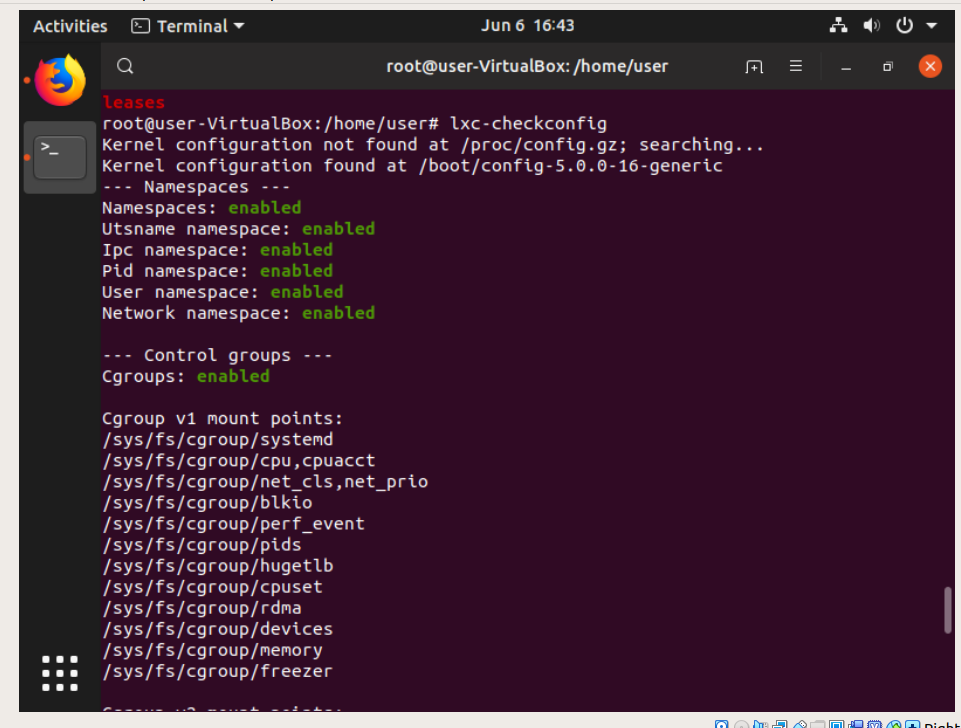
\includegraphics[scale=0.30]{P91.png}\\
        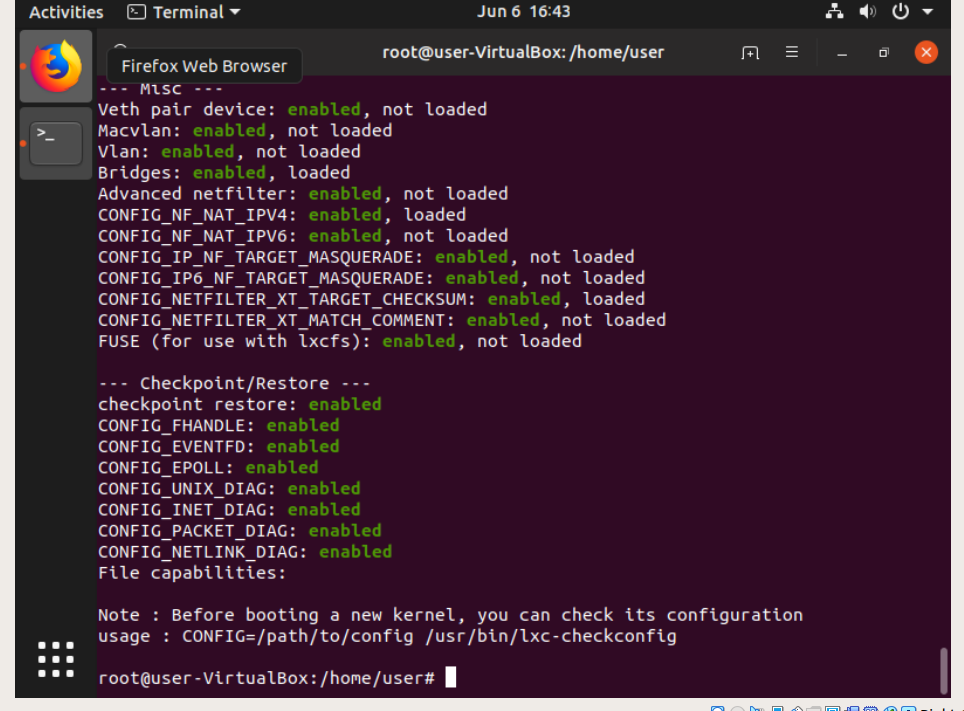
\includegraphics[scale=0.30]{P92.png}
    \end{center}
    \item Ahora debemos obtener los subuids y subgids del usuario de lxc con el siguiente comando(user se llama nuestro usuario sin privilegios):
    \begin{verbatim}
        sudo grep user /etc/sub{gid,uid}
    \end{verbatim}
    \begin{center}
        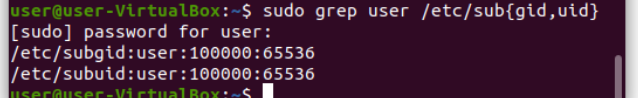
\includegraphics[scale=0.45]{P93.png}
    \end{center}
    \item ahora con cualquier editor de texto agregamos la siguiente linea:
    \begin{verbatim}
        user veth lxcbr0 10
    \end{verbatim}
    En el directorio $/etc/lxc/lxc-usernet$ esto para que el usuario tenga permitido crear hasta 10 dispositivos de tipo veth y agregarlos al puente llamado lxcbr0.
    \begin{center}
        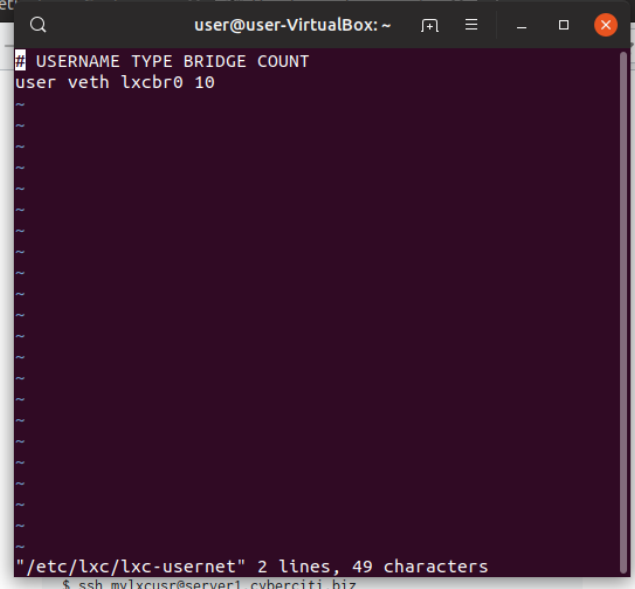
\includegraphics[scale=0.45]{P94.png}
    \end{center}
    \item Una vez hecho lo anterior lo que debemos hacer es crear el siguiente directorio:
    \begin{verbatim}
        mkdir -p ~/.config/lxc
    \end{verbatim}
    Y vamos a crear el archivo de configuración copiando lo siguiente:
    \begin{verbatim}
 cp /etc/lxc/default.conf ~/.config/lxc/default.conf
    \end{verbatim}
    \begin{center}
        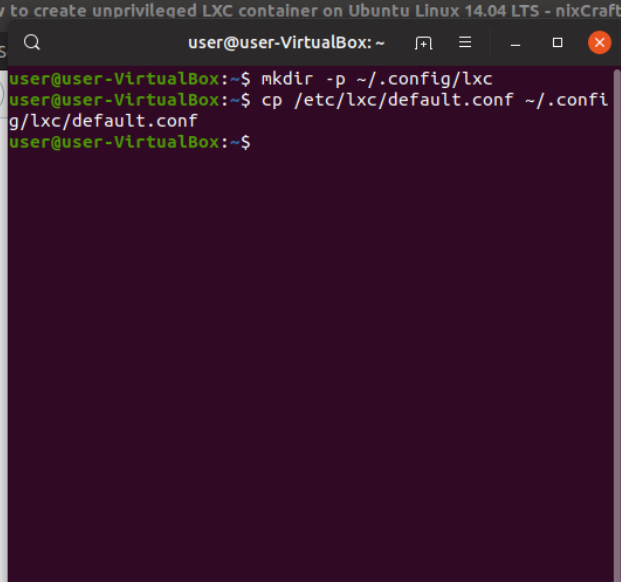
\includegraphics[scale=0.45]{p95.png}
    \end{center}
    \item Utilizando el editor te texto que sea vamos a abrir el siguiente archivo $~/.config/lxc/default.conf$ y agregamos las siguientes lineas(basado en las Id's que obtuvimos anteriormente):
    \begin{verbatim}
        lxc.id_map = u 0 100000 65536
        lxc.id_map = g 0 100000 65536
    \end{verbatim}
    \begin{center}
        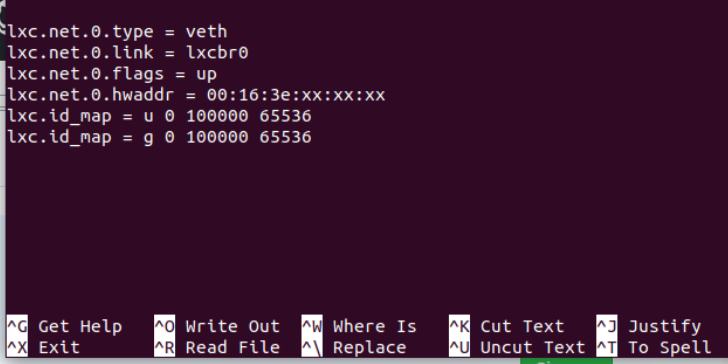
\includegraphics[scale=0.40]{P966.png}
    \end{center}
    \item Terminados los pasos anteriores procedemos a crear nuestro contenedor:\\
    lxc-create -t download -n contenedorcentos $--$ -d centos -r 7 -a amd64
    \begin{center}
        
\includegraphics[scale=0.35]{contenedor.png}
    \end{center}
    \end{itemize}
    
\end{itemize}
\end{document}